\documentclass{article}

\usepackage{graphicx}
\usepackage{subfigure}
\usepackage[hypcap]{caption}
\usepackage{listings}
\usepackage{float}
\floatstyle{plaintop}
\restylefloat{table}

\title{Experimental Design and Data Analysis: Assignment 4}
\author{Andrew Bedard(2566978) \& Simone van Gompel(2567525) \\ Group 19}

\begin{document}

  \maketitle

  \section*{Exercise 1}
    \subsection*{1}
      \begin{lstlisting}[language=R]
      sample_slices = sample(1:18, 18)
      \end{lstlisting}
    
    \subsection*{2}
      \begin{figure}[H]
          \centering
          \subfigure[Humidity]
          {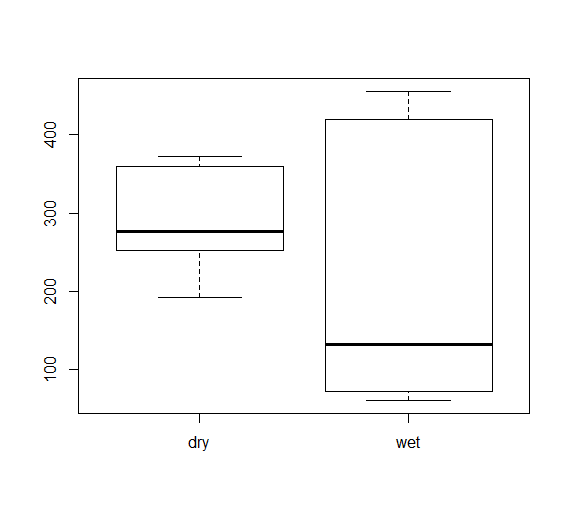
\includegraphics[scale=0.2]{../results/BoxHoursHum.png} }
          \subfigure[Environment]
          {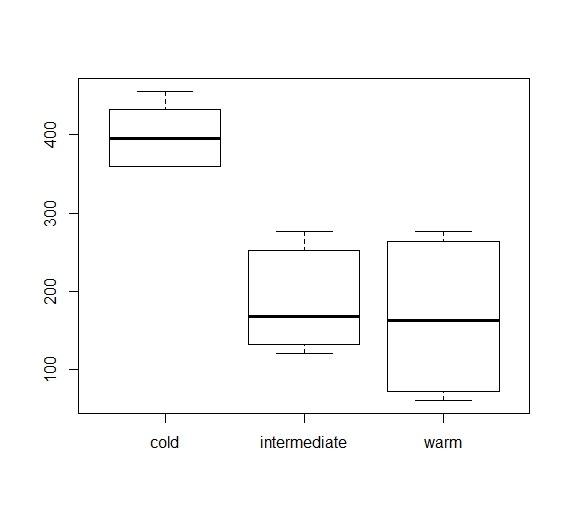
\includegraphics[scale=0.2]{../results/BoxHoursEnv.png} }
          \caption{Boxplots of Hours with Humidity and Environment}
          \label{fig:BoxHours}
      \end{figure} 
    
    \subsection*{3}
      \begin{figure}[H]
          \centering
          \subfigure[Humidity]
          {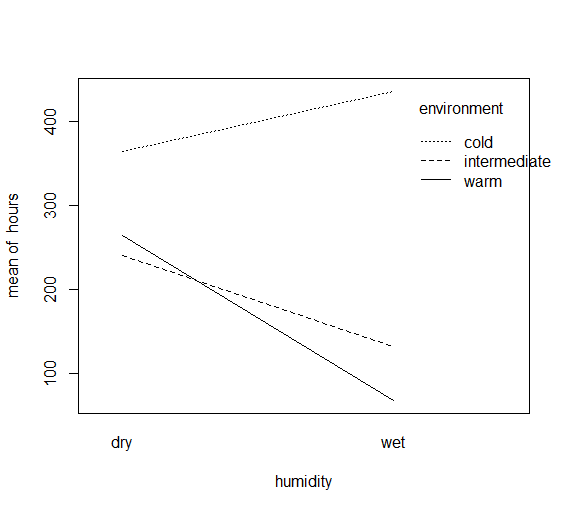
\includegraphics[scale=0.2]{../results/IntPlotHoursHum.png} }
          \subfigure[Environment]
          {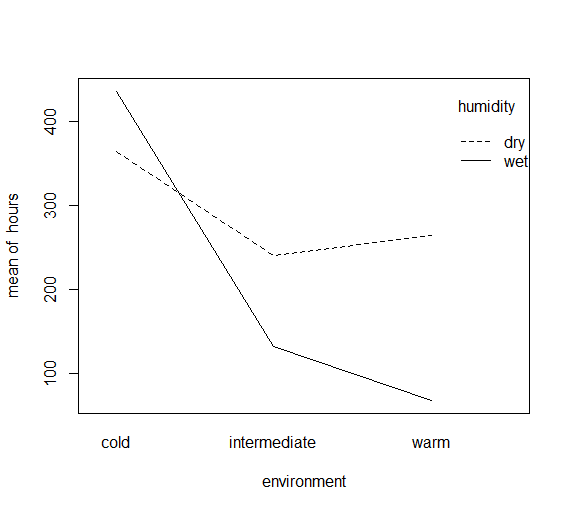
\includegraphics[scale=0.2]{../results/IntPlotHoursEnv.png} }
          \caption{Interactionplots of Hours with Humidity and Environment}
          \label{fig:IntPlotHours}
      \end{figure}
    
    \subsection*{4}
      Analysis of variance on both factors:\\\\
      \begin{lstlisting}[language=R]
Analysis of Variance Table

Response: hours
            Df Sum Sq Mean Sq F value    Pr(>F)    
environment  2 201904  100952 23.1057 3.674e-05 ***
humidity     1  26912   26912  6.1596   0.02637 *  
Residuals   14  61168    4369                      
---
Signif. codes:  0 ‘***’ 0.001 ‘**’ 0.01 ‘*’ 0.05 ‘.’ 0.1 ‘ ’ 1
      \end{lstlisting}
    
    \subsection*{5}
    
    \subsection*{6}
    
    \subsection*{7}
    
    \subsection*{8}
    
  \section*{Exercise 2}
    \subsection*{1}
     
    \subsection*{2}
	\begin{figure}[H]
		\centering
          \subfigure[]
          {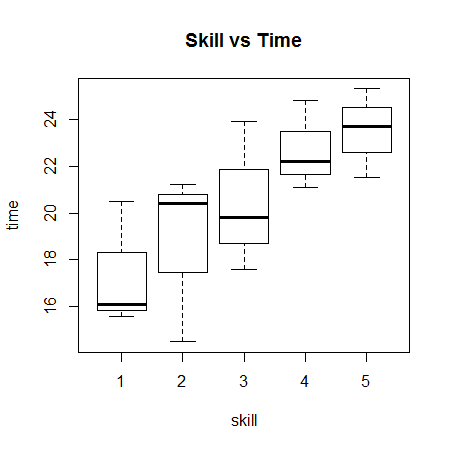
\includegraphics[scale=0.35]{../results/2_2_1.png} }
          \subfigure[]
          {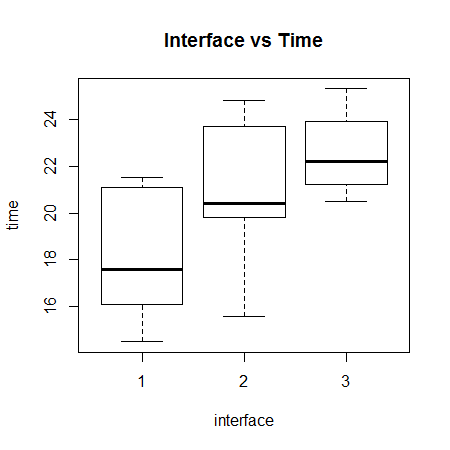
\includegraphics[scale=0.35]{../results/2_2_2.png} }
          \caption{Box Plots of Skill and Interface vs Time}
          \label{fig:srchbox}
	\end{figure}
	
	\begin{figure}[H]
	\centering
		\subfigure[]
          {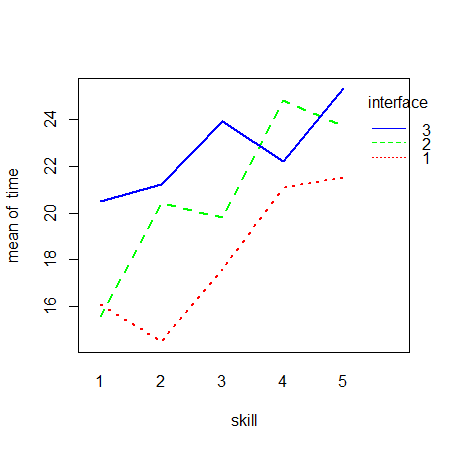
\includegraphics[scale=0.35]{../results/2_2_3.png} }
          \subfigure[]
          {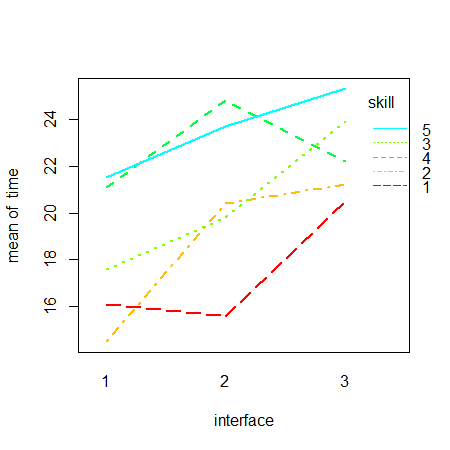
\includegraphics[scale=0.35]{../results/2_2_4.png} }
          \caption{Interaction plots of Skill and Interface vs Time}
          \label{fig:srch_interaction}
	\end{figure}
	
	It is difficult to conclude that there is an interaction between skill and interface as they are clearly not parallel, but they follow the same general trajectory, so this interaction may be due to noise. 
    \subsection*{3}
    Using the Kurskal-Wallis rank sum test, we test if the distributions of our populations in regards to the time measured for different interfaces are the same, and we obtain the following results:\\\\
      \begin{lstlisting}[language=R]
Kruskal-Wallis rank sum test

data: time and interface
Kruskal-Wallis chi-squared = 4.22, df = 2, p-value =0.1212
      \end{lstlisting}
      Thus with a p-value of 0.1212 we reject the null hypothesis that our populations are the same, therefore the search time for all interfaces is not equal.
    \subsection*{4}
    
    \subsection*{5}
    \begin{figure}[H]
    \centering
    	\subfigure[]
		{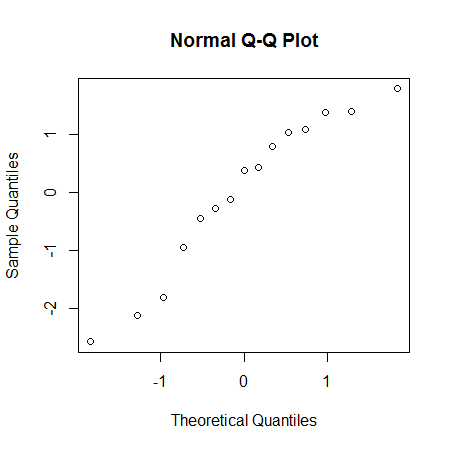
\includegraphics[scale=0.35]{../results/2_5_1.png} }
        \subfigure[]
        {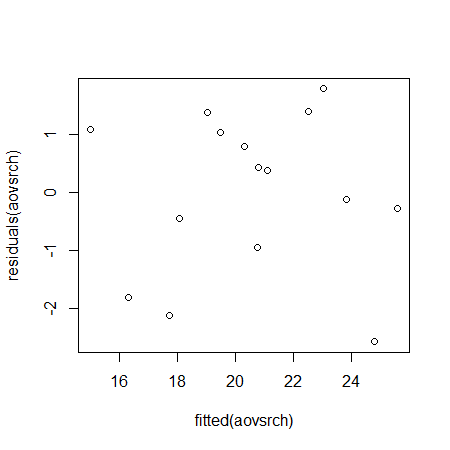
\includegraphics[scale=0.35]{../results/2_5_2.png} }
        \caption{Diagnostic Plots}
        \label{fig:diagnostic}
    \end{figure}
    It is difficult to say for certain, there may be a slight curve in the qq-plot \ref{fig:diagnostic}(a) but it looks approximately normal, and the fitted value plot \ref{fig:diagnostic}(b) suggests there is no significant difference in the population variances.
    \subsection*{6}
    
    \subsection*{7}
    
  \section*{Exercise 3}
    \subsection*{1}
    
    \subsection*{2}
    
    \subsection*{3}
    
    \subsection*{4}
    
    \subsection*{5}
    
  \section*{Exercise 4}
    \subsection*{1}
    
    \subsection*{2}
    
    \subsection*{3}
    
    \subsection*{4}

    
  \section{R-Code}
    \subsection{Exercise 1}\label{sec:RE1}
      \begin{lstlisting}[language=R]
      \end{lstlisting}
    \subsection{Exercise 2}\label{sec:RE2}
      \begin{lstlisting}[language=R]
      \end{lstlisting}
    \subsection{Exercise 3}\label{sec:RE3}
      \begin{lstlisting}[language=R]
      \end{lstlisting}
    \subsection{Exercise 4}\label{sec:RE4}
      \begin{lstlisting}[language=R]
      \end{lstlisting}
\end{document}
